{
\begin{figure}
    \centering
    \begin{subfigure}[t]{0.25\textwidth}
        \centering
        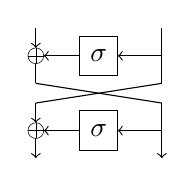
\begin{tikzpicture}[xscale=0.8, yscale=-0.5]
            \draw [->] (0,0) -- (0,0.5);
            \draw [very thin] (0,0.7) ellipse (0.125 and 0.2);
            \draw [very thin] (0,0.5) -- (0,0.9);
            \draw [very thin] (-0.125,0.7) -- (0.125,0.7);
            \draw (2,0) -- (2,0.7);
            \draw [->] (2,0.7) -- (1.3,0.7);
            \draw (0.7,0.2) rectangle (1.3,1.2) node[pos=0.5] {$\sigma$};
            \draw [->] (0.7,0.7) -- (0.125,0.7);
            \draw (0,0.9) -- (0,1.4);
            \draw (2,0.7) -- (2,1.4);
            \draw (2,1.4) -- (0,1.9);
            \draw (0,1.4) -- (2,1.9);
            \draw [->] (0,1.9) -- (0,2.4);
            \draw [very thin] (0,2.6) ellipse (0.125 and 0.2);
            \draw [very thin] (0,2.4) -- (0,2.8);
            \draw [very thin] (-0.125,2.6) -- (0.125,2.6);
            \draw (2,1.9) -- (2,2.6);
            \draw [->] (2,2.6) -- (1.3,2.6);
            \draw (0.7,2.1) rectangle (1.3,3.1) node[pos=0.5] {$\sigma$};
            \draw [->] (0.7,2.6) -- (0.125,2.6);
            \draw [->] (0,2.8) -- (0,3.3);
            \draw [->] (2,2.6) -- (2,3.3);
        \end{tikzpicture}
        \caption{\label{fig.central-sigma}The linear layer from the decomposition}
    \end{subfigure}
    \hspace{0.5cm}
    \begin{subfigure}[t]{0.3\textwidth}
        \centering
        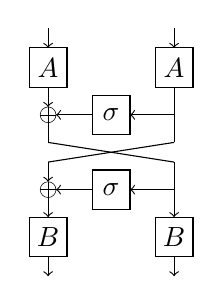
\begin{tikzpicture}[xscale=0.8, yscale=-0.5]
            \draw [->] (0,0) -- (0,0.5);
            \draw (-0.3,0.5) rectangle (0.3,1.5) node[pos=0.5] {$A$};
            \draw [->] (2,0) -- (2,0.5);
            \draw (1.7,0.5) rectangle (2.3,1.5) node[pos=0.5] {$A$};
            \draw [->] (0,1.5) -- (0,2);
            \draw [very thin] (0,2.2) ellipse (0.125 and 0.2);
            \draw [very thin] (0,2) -- (0,2.4);
            \draw [very thin] (-0.125,2.2) -- (0.125,2.2);
            \draw (2,1.5) -- (2,2.2);
            \draw [->] (2,2.2) -- (1.3,2.2);
            \draw (0.7,1.7) rectangle (1.3,2.7) node[pos=0.5] {$\sigma$};
            \draw [->] (0.7,2.2) -- (0.125,2.2);
            \draw (0,2.4) -- (0,2.9);
            \draw (2,2.2) -- (2,2.9);
            \draw (2,2.9) -- (0,3.4);
            \draw (0,2.9) -- (2,3.4);
            \draw [->] (0,3.4) -- (0,3.9);
            \draw [very thin] (0,4.1) ellipse (0.125 and 0.2);
            \draw [very thin] (0,3.9) -- (0,4.3);
            \draw [very thin] (-0.125,4.1) -- (0.125,4.1);
            \draw (2,3.4) -- (2,4.1);
            \draw [->] (2,4.1) -- (1.3,4.1);
            \draw (0.7,3.6) rectangle (1.3,4.6) node[pos=0.5] {$\sigma$};
            \draw [->] (0.7,4.1) -- (0.125,4.1);
            \draw [->] (0,4.3) -- (0,4.8);
            \draw (-0.3,4.8) rectangle (0.3,5.8) node[pos=0.5] {$B$};
            \draw [->] (2,4.1) -- (2,4.8);
            \draw (1.7,4.8) rectangle (2.3,5.8) node[pos=0.5] {$B$};
            \draw [->] (0,5.8) -- (0,6.3);
            \draw [->] (2,5.8) -- (2,6.3);
        \end{tikzpicture}
        \caption{\label{fig.linear-feistel-1}Applying arbitrary linear bijections $A$ and $B$}
    \end{subfigure}
    \hspace{0.5cm}
    \begin{subfigure}[t]{0.32\textwidth}
        \centering
        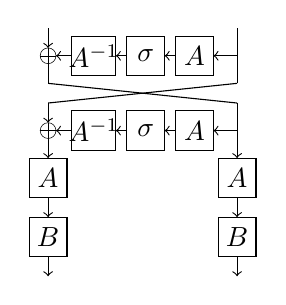
\begin{tikzpicture}[xscale=0.8, yscale=-0.5]
            \draw [->] (0,0) -- (0,0.5);
            \draw [very thin] (0,0.7) ellipse (0.125 and 0.2);
            \draw [very thin] (0,0.5) -- (0,0.9);
            \draw [very thin] (-0.125,0.7) -- (0.125,0.7);
            \draw (3,0) -- (3,0.7);
            \draw [->] (3,0.7) -- (2.625,0.7);
            \draw (2.025,0.2) rectangle (2.625,1.2) node[pos=0.5] {$A$};
            \draw [->] (2.025,0.7) -- (1.85,0.7);
            \draw (1.25,0.2) rectangle (1.85,1.2) node[pos=0.5] {$\sigma$};
            \draw [->] (1.25,0.7) -- (1.075,0.7);
            \draw (0.375,0.2) rectangle (1.075,1.2) node[pos=0.5] {$A^{-1}$};
            \draw [->] (0.375,0.7) -- (0.125,0.7);
            \draw (0,0.9) -- (0,1.4);
            \draw (3,0.7) -- (3,1.4);
            \draw (3,1.4) -- (0,1.9);
            \draw (0,1.4) -- (3,1.9);
            \draw [->] (0,1.9) -- (0,2.4);
            \draw [very thin] (0,2.6) ellipse (0.125 and 0.2);
            \draw [very thin] (0,2.4) -- (0,2.8);
            \draw [very thin] (-0.125,2.6) -- (0.125,2.6);
            \draw (3,1.9) -- (3,2.6);
            \draw [->] (3,2.6) -- (2.625,2.6);
            \draw (2.025,2.1) rectangle (2.625,3.1) node[pos=0.5] {$A$};
            \draw [->] (2.025,2.6) -- (1.85,2.6);
            \draw (1.25,2.1) rectangle (1.85,3.1) node[pos=0.5] {$\sigma$};
            \draw [->] (1.25,2.6) -- (1.075,2.6);
            \draw (0.375,2.1) rectangle (1.075,3.1) node[pos=0.5] {$A^{-1}$};
            \draw [->] (0.375,2.6) -- (0.125,2.6);
            \draw [->] (0,2.8) -- (0,3.3);
            \draw (-0.3,3.3) rectangle (0.3,4.3) node[pos=0.5] {$A$};
            \draw [->] (3,2.6) -- (3,3.3);
            \draw (2.7,3.3) rectangle (3.3,4.3) node[pos=0.5] {$A$};
            \draw [->] (0,4.3) -- (0,4.8);
            \draw (-0.3,4.8) rectangle (0.3,5.8) node[pos=0.5] {$B$};
            \draw [->] (3,4.3) -- (3,4.8);
            \draw (2.7,4.8) rectangle (3.3,5.8) node[pos=0.5] {$B$};
            \draw [->] (0,5.8) -- (0,6.3);
            \draw [->] (3,5.8) -- (3,6.3);
        \end{tikzpicture}
        \caption{\label{fig.linear-feistel-2}Moving the linear functions $A$ down}
    \end{subfigure}
    \FigDef{modifying-feistel}{Propagation of the linear function $A$ through the middle linear layer.}
\end{figure}
}